\documentclass[tikz]{standalone}
\date{}
\usepackage{amsmath,amsthm,amssymb}
\usepackage{xcolor}
\usepackage{tikz}
\usepackage[siunitx]{circuitikz}
\usepackage{tikz-3dplot}
\usepackage{ifthen}
\tikzset{isometricXYZ/.style={x={(-0.866cm,-0.5cm)}, y={(0.866cm,-0.5cm)}, z={(0cm,1cm)}}}
\usetikzlibrary{arrows,decorations.pathmorphing,positioning,fit,trees,shapes,automata,calc,intersections,decorations.markings,patterns,graphs,quotes,plotmarks}
%\usepackage{algorithm}
%\usepackage{algorithmic}
\newcommand{\R}{\mathbb{R}}
\newcommand{\F}{\mathbb{F}}
\newcommand{\bmat}[1]{\begin{bmatrix}#1\end{bmatrix}}
\newcommand{\xth}[1]{{#1}^{\mathrm{th}}}
\newcommand{\pd}[2]{\frac{\partial #1}{\partial #2} }
\newcommand{\pdd}[2]{\frac{\partial^2 #1}{\partial #2^2}}
\newcommand{\myitemsep}{\setlength\itemsep{-0.25em}}
\newcommand{\bigpar}[1]{\left( #1\right)}
\tikzset{myedge/.style={ thick,->,>=stealth',inner sep=0pt,outer sep=3pt}}
\tikzset{hv path/.style= {to path={-| (\tikztotarget)}}}
\tikzset{vh path/.style= {to path={|- (\tikztotarget)}}}

%%%%%%%%%% Using shift and rotate around:

\newcommand{\spring}[4]{
\path[shift={#1},rotate={#2},fill = white,opacity=1.0] (-0.25,-0.5) rectangle (0.25,0.5); % cover
\draw[thick,shift={#1},rotate={#2}] (0,0.5) -- +(0.25,-0.1) -- +(-0.25,-0.2)-- +(0.25,-0.3)-- +(-0.25,-0.4)-- +(0.25,-0.5)-- +(-0.25,-0.6)-- +(0.25,-0.7)-- +(-0.25,-0.8)-- +(0.25,-0.9) -- +(0,-1.0);
\draw[thick,shift={#1},rotate={#2}] (#3,0) node {#4};
}
\newcommand{\ground}[3]{
\draw[thick,shift={#1},rotate={#2}] (-0.5*#3cm,0) -- (0.5*#3cm,0);
\path[thick,shift={#1},rotate={#2},pattern=north west lines] (-0.5*#3cm,0) rectangle (0.5*#3cm,0.2);
}
\newcommand{\dashpot}[4]{
\path[shift={#1},rotate={#1},fill = white,opacity=1.0] (-0.25,0) rectangle (0.25,0.15);
\path[shift={#1},rotate={#1},draw,thick] (0,0) -- +(0.25,0) -- +(0.25,0.25) +(0.15,0.15) -- +(-0.15,0.15)  +(-0.25,0.25) -- +(-0.25,0) -- +(0,0);
\draw[thick,shift={#1},rotate={#1}] (#3,0) node {#4};
}
\newcommand{\mydashpot}[5]{
\begin{scope}[xshift=#1cm,yshift=#2cm,rotate=#3]
	\path[fill = white,opacity=1.0] (-0.25,0) rectangle (0.25,0.15);
	\path[draw,thick] (0,0) -- +(0.25,0) -- +(0.25,0.25) +(0.15,0.15) -- +(-0.15,0.15)  +(-0.25,0.25) -- +(-0.25,0) -- +(0,0);
	\node at (#4,0) {#5};
	\end{scope}
}
\newcommand{\lapof}[1]{\mathcal L \left\{ #1 \right\}}
\newcommand{\lapinv}[1]{\mathcal L^{-1} \left\{ #1 \right\}}
\newcommand{\evalat}[2]{\left. #1 \right|_{#2}}
\newcommand{\myarr}[3]{(-#2:#1) arc (-#2:#2:#1) node[#3] }
\newcommand{\mc}[1]{\mathcal{#1}}
\newcommand{\mred}[1]{\textcolor{red}{[#1]}}
\newcommand{\myco}[2]{\bigpar{ \frac{#1}{#2} }}
\newcommand{\tc}[2]{{#1}{#2}}
\newcommand{\mcb}[1]{{\color{blue}#1}}
\newcommand{\mcr}[1]{{\color{red}#1}}
\newcommand{\mcg}[1]{{\color{green!70!black}#1}}
\usepackage{hyperref}
\hypersetup{colorlinks=true,
linkcolor=blue,          % color of internal links
        citecolor=green,        % color of links to bibliography
          filecolor=magenta,      % color of file links
           urlcolor=blue           % color of external links
}

\usetikzlibrary{shapes.misc}

\tikzset{nonterminal/.style={
  % The shape:
  rectangle,
  % The size:
  minimum size=6mm,
  % The border:
  very thick,
  draw=red!50!black!50,
  % The filling:
  top color=white,
  bottom color=red!50!black!20,
  % Font:
  font=\itshape,
  }
}

\tikzset{terminal/.style={
  % The shape:
  rounded rectangle,
  minimum size=6mm,
  % The rest
  very thick,draw=black!50,
  top color=white,bottom color=black!20,
  font=\ttfamily,
  }
}



\begin{document}


\begin{tikzpicture}[node distance=5mm]
  \node [nonterminal] {unsigned integer};
\end{tikzpicture}


\begin{tikzpicture}[node distance=5mm,
        text height=1.5ex,text depth=0.25em
  ]
  \node (dot)   [terminal]                {.};
  \node (digit) [terminal,right=of dot]   {digit};
  \node (E)     [terminal,right=of digit] {E};
\end{tikzpicture}


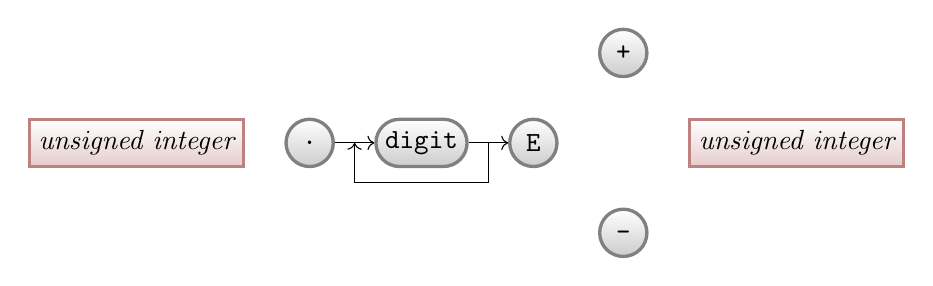
\begin{tikzpicture}[
    node distance=5mm and 5mm,
    terminal/.append style={rectangle,rounded corners=3mm},
    skip loop/.style={to path={-- ++(0,#1) -| (\tikztotarget)}}
  ]
  \node (ui1)   [nonterminal]                      {unsigned integer};
  \node (dot)   [terminal,right=of ui1]            {.};
  \node (digit) [terminal,right=of dot]            {digit};
  \node (E)     [terminal,right=of digit]          {E};
  \node (plus)  [terminal,above right=of E]        {+};
  \node (minus) [terminal,below right=of E]        {-};
  \node (ui2)   [nonterminal,below right=of plus]  {unsigned integer};

  \path (dot)   edge[->]                   (digit)  % simple edges
        (digit) edge[->]                   (E)
        ($ (digit.east)!0.5!(E.west) $)
                edge[->,skip loop=-5mm] ($ (digit.west)!0.5!(dot.east) $);
\end{tikzpicture}


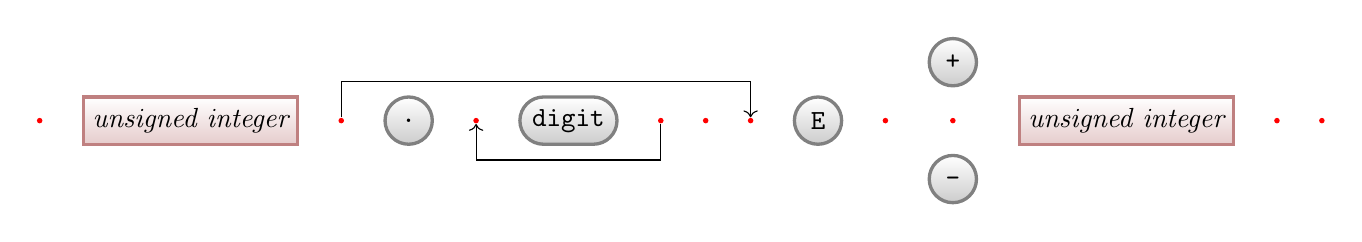
\begin{tikzpicture}[point/.style={circle,inner sep=0pt,minimum
        size=2pt,fill=red}, skip loop/.style={to path={-- ++(0,#1) -|
        (\tikztotarget)}}]
  \matrix[row sep=1mm,column sep=5mm] {
    % First row:
      & & & & & & & & & & & \node (plus) [terminal] {+}; \\
    % Second row:
    \node (p1) [point]  {}; &    \node (ui1)   [nonterminal] {unsigned integer}; &
    \node (p2) [point]  {}; &    \node (dot)   [terminal]    {.};                &
    \node (p3) [point]  {}; &    \node (digit) [terminal]    {digit};            &
    \node (p4) [point]  {}; &    \node (p5)    [point]  {}; &    
    \node (p6) [point]  {}; &    \node (e)     [terminal]    {E};                &
    \node (p7) [point]  {};                                                      &
    \node (p8) [point]  {}; &    \node (ui2)   [nonterminal] {unsigned integer}; & 
    \node (p9) [point]  {}; &    \node (p10)   [point]       {};\\
    % Third row:
    & & & & & & & & & & & \node (minus) [terminal] {-};\\
  };

  \path (p4) edge [->,skip loop=-5mm] (p3)
        (p2) edge [->,skip loop=5mm]  (p6);
\end{tikzpicture}

\end{document}
